\chapter{Architecture}
\label{sec:architecture}

The \gls{vurm} virtualization capabilities have to be integrated with the existing \gls{slurm} job scheduler in order to exploit the functionalities offered by each component. At least a basic understanding of the \gls{slurm} internals is thus needed in order to design the best possible architecture for the \gls{vurm} utility. This chapter aims to introduce the reader to both the \gls{slurm} and \gls{vurm} architectural design and explains the reasons behind the different choices that led to the implemented solution.

The content presented in this chapter is structured into the following sections:

\begin{itemize}
	\item Section \ref{sec:slurm-arch} introduces the \gls{slurm} architecture and explains the details needed to understand how \gls{vurm} integrates into the system;
	\item Section \ref{sec:vurm-arch} explains the chosen \gls{vurm} architecture and presents the design choices that led to the final implementation;
	\item Section \ref{sec:vc-creation} introduces the provisioning workflow used to allocate new resources to users requesting them and introduces the concept of \emph{virtual clusters};
	\item Section \ref{sec:new-provisioners} explains the details of the implementation of a new resource provisioner and its integration in a \gls{vurm} system.
\end{itemize}



\section{SLURM architecture}
\label{sec:slurm-arch}

The architecture of the \gls{slurm} batch scheduler was conceived to be easily expandable and customizable, either by configuring it the right way or by adding functionalities through the use of specific plugins.

This section does not aim to provide a complete understanding of how the \gls{slurm} internals are implemented or which functionalities can be extended through the use of plugins; it will be limited instead to providing a global overview of the different entities which intervene in its very basic lifecycle and which are needed to understand the \gls{vurm} architecture presented afterwards.


\subsection{Components}

A basic overview of the \gls{slurm} architecture is presented in \autoref{fig:slurm-arch}. Note that the actual architecture is much more complex than what illustrated in the class diagram and involves different additional entities (such as backup controllers, databases,…) and interactions. Although, for the scope of this project, the representation covers all the important parts and can be used to place the \gls{vurm} architecture in the right context later on in this chapter.

\begin{figure}[ht]
	\centering
	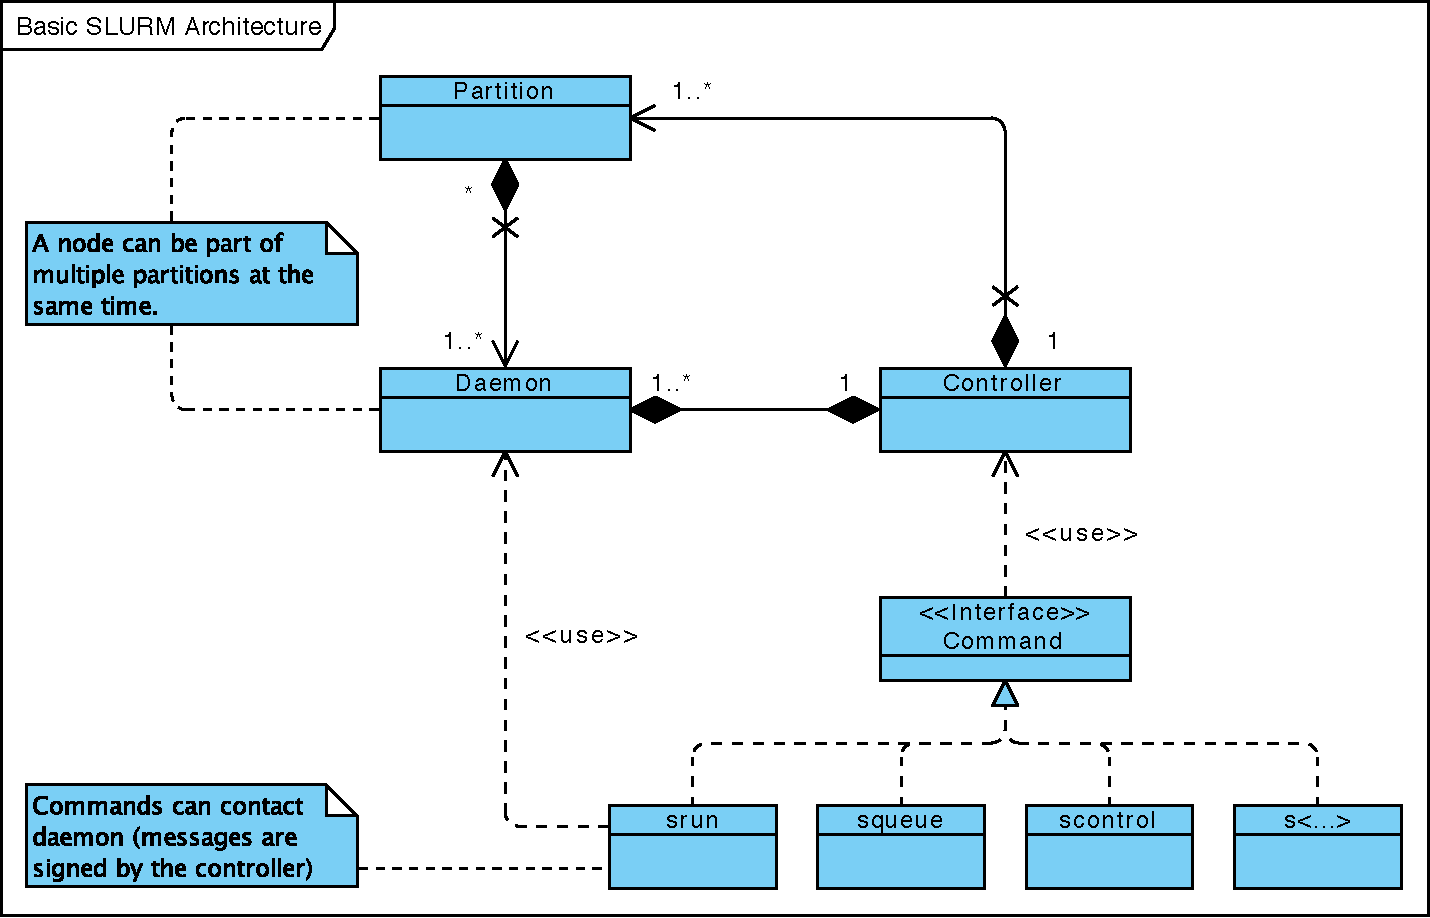
\includegraphics[width=0.9\textwidth]{figures/basic-slurm-arch}
	\caption{Basic overview of the SLURM architecture}
	\label{fig:slurm-arch}
\end{figure}

The classes represented in the diagram are not directly mapped to actual objects in the \gls{slurm} codebase, but rather to the different intervening entities\footnote{A deployment diagram may be more suitable for this task, but a class diagram allows to better represent the cardinality of the relationships between the different entities.}; the rest of this subsection is dedicated to provide some more explications about them.

\subsubsection{Controller}
The \texttt{Controller} class represents a single process controlling the whole system; its main responsibility is to schedule incoming jobs and assign them to nodes for execution based on different (configurable) criteria. Additionally, it keeps track of the state of each configured daemon and partition, accepts incoming administration requests and maintains an accounting database.

A \emph{backup} controller can also be defined; requests are sent to this controller instead of the main one as soon as a requesting client notices that the main controller is no more able to correctly process incoming requests.

Optionally, a \gls{dbms} backend can be used to take advantage of additional functionalities such as per-user accounting or additional logging.

\subsubsection{Daemons}
Each \texttt{Daemon} class represents a process running on a distinct node; their main task is to accept incoming job requests and run them on the local node.

The job execution commands (see below) communicate with the daemons directly after having received an allocation token by the controller. The first message they send to the nodes to request job allocation and/or execution is signed by the controller. This decentralized messaging paradigm allows for better scalability on clusters with many nodes as the controller does not have to deal with the job execution processing on each node itself.

Each daemon is periodically pinged by the controller to maintain its status updated in the central node database.

\subsubsection{Partitions}
The \texttt{Daemon} instances (and thus the nodes) are organized in one or more (possibly overlapping) logical partitions; each partition can be configured individually with regard to permissions, priorities, maximum job duration, etc. This allows to create partitions with different settings. A possible example of useful per-partition configuration is to allow only a certain group of users to access a partition which contains more powerful nodes. Another possible example is to organize the same set of nodes in two overlapping partitions with different priorities; jobs submitted to the partition with higher priority will thus be carried out faster (i.e. their allocation will have an higher priority) than jobs submitted to the partition with lower priority.

\subsubsection{Commands}
Different \texttt{Command}s are made available to administrators and end users; they communicate with the \texttt{Controller} (and possibly directly with the \texttt{Daemon}s) by using a custom binary protocol and TCP/IP as the transport layer.

The main commands used throughout the project are the \texttt{srun} command, which allows to submit a job for execution (and offers a plethora of options and arguments to fine tuning the request) and the \texttt{scontrol} command, which can be used to perform administration requests, as for example listing all nodes or reloading the configuration file.


\subsection{Configuration}

The \gls{slurm} configuration resides in one single file which exposes a simple syntax. This configuration file contains the directives for all components of a SLURM-managed system (including thus the controller, the daemons, the databases,…); an excerpt of such a file is showed in \autoref{lst:conf-example}.

\lstset{language=bash,caption=Configuration excerpt,label=lst:conf-example}
\begin{lstlisting}
# slurm.conf file generated by configurator.html.
# Put this file on all nodes of your cluster.
# See the slurm.conf man page for more information.
#
ControlMachine=controller-hostname
# ...
SlurmctldPidFile=/var/run/slurmctld.pid
SlurmctldPort=6817
SlurmdPidFile=/var/run/slurmd.pid
SlurmdPort=6818
SlurmdSpoolDir=/tmp/slurmd
SlurmUser=nelson
# ...
NodeName=testing-node Procs=1 State=UNKNOWN
PartitionName=debug Nodes=ubuntu Default=YES MaxTime=INFINITE State=UP

NodeName=nd-6ad4185-0 NodeHostname=10.0.0.101
NodeName=nd-6ad4185-1 NodeHostname=10.0.0.100
PartitionName=vc-6ad4185 Nodes=nd-6ad4185-[0-1] Default=NO MaxTime=INFINITE State=UP
\end{lstlisting}

An important feature of the \gls{slurm} controller daemon is its ability to reload this configuration file at runtime. This feature is exploited to dynamically add or remove nodes and partitions from a running system. The file can be reloaded by executing a simple administration request through the use of the \texttt{scontrol} command, as illustrated in the \autoref{lst:reconfig}.

\lstset{language=bash,caption=Reconfiguration command,label=lst:reconfig}
\begin{lstlisting}
$ scontrol reconfigure
\end{lstlisting}

A useful feature leveraged by the configuration syntax is the ability to group node definitions if their \texttt{NodeName} is terminated by numerical indexes; this may not be deemed that interesting when working with 10 nodes, but being able to group configuration directives for clusters of thousands of nodes may be more than welcome. The listings \ref{lst:node-no-grouping} and \ref{lst:node-grouping} show an example of this feature.

\lstset{language=bash,caption=Node naming without grouping,label=lst:node-no-grouping}
\begin{lstlisting}
NodeName=linux1 Procs=1 State=UNKNOWN
NodeName=linux2 Procs=1 State=UNKNOWN
# ... 29 additional definitions ...
NodeName=linux32 Procs=1 State=UNKNOWN
PartitionName=debug Nodes=linux1,linux2,...,linux32 Default=YES MaxTime=INFINITE State=UP
\end{lstlisting}

\lstset{language=bash,caption=Node naming with grouping,label=lst:node-grouping}
\begin{lstlisting}
NodeName=linux[1-32] Procs=1 State=UNKNOWN
PartitionName=debug Nodes=linux[1-32] Default=YES MaxTime=INFINITE State=UP
\end{lstlisting}

\section{VURM architecture}
\label{sec:vurm-arch}

The previous section introduced some of the relevant \gls{slurm} architectural concepts. This section, instead, aims to provide an overview of the final implemented solution and the process that led to the architectural design of the \gls{vurm} framework.

\rule[.15em]{10pt}{.3pt} \textbf{\tiny NOTE 1 }{\leaders\hbox{\rule[.15em]{1pt}{.3pt}}\hfill}

\vspace*{-2.5mm}\begin{list}{·}{\leftmargin=1em}
	%\setlength{\itemsep}{-2mm}
	\item Blue circles represent virtual machines (blue color is used for virtual resources or software running on virtual resources).
	\item Green squares represent physical nodes (green color is used for physical resources or software running on physical resources).
	\item Virtual machines and physical nodes can be grouped into virtual clusters and partitions respectively.
	\item Rounded rectangles represent services or programs.
\end{list}
\vspace*{-4.5mm}\rule{\textwidth}{.3pt}

\rule[.15em]{10pt}{.3pt} \textbf{\tiny NOTE 2 }{\leaders\hbox{\rule[.15em]{1pt}{.3pt}}\hfill}
\\[1mm]
The term \emph{Virtual Clusters} is used a couple of times here. For now, consider a virtual cluster only as a \gls{slurm} partition with a label attached to it; the \autoref{sec:vc-creation} contains more information about these special partitions.

\vspace*{-4.5mm}\rule{\textwidth}{.3pt}

\subsection{A first proposal}

The first approach chosen to implement the \gls{vurm} architecture was to use \gls{slurm} for everything and inject the needed virtualization functionalities into it, either by adding plugins or modifying the original source code. This approach is introduced by the \autoref{fig:vurm-arch-top}. To help better understand the different parts, the representation splits the architecture on two different layers: a physical layer and a virtual layer.

\begin{figure}[ht]
	\centering
	\includegraphics[width=0.7\textwidth]{figures/vurm-arch-bottom-up}
	\caption{Initial proposal for the VURM architecture}
	\label{fig:vurm-arch-top}
\end{figure}

In this proposal, physical nodes (each node runs a \gls{slurm} daemon) are managed by the \gls{slurm} controller. When a new request is received by the controller a new \gls{vm} is started on one of these nodes and a \gls{slurm} daemon setup and started on it. Upon startup this daemon registers itself as a new node to the \gls{slurm} controller. Once the registration occurred, the \gls{slurm} controller can then allocate resources and submit jobs to the new virtual node.

The initial idea behind this proposal was to spawn new virtual machines by running a job which takes care of this particular task through the \gls{slurm} system itself. This job will be run on a daemon placed inside the \emph{seed partition}.

The \gls{slurm} controller daemon can't, in this case, differentiate between daemons running on physical or virtual nodes. It only knows that to spawn new virtual machines, the respective job has to be submitted to the \emph{seed partition}, while user jobs will be submitted to one of the created \emph{virtual cluster} partitions. In this case  the user has to specify in which virtual cluster (i.e. in which partition) he wants to run the job.

The \autoref{fig:slurm-pov} illustrates how the \gls{slurm} controller sees the whole system (note that virtual and physical nodes as well as virtual clusters and partition are still differentiated for illustration purposes, but aside their name the \gls{slurm} controller isn't able to tell the differences between them).

\begin{figure}[ht]
	\centering
	\includegraphics[width=0.8\textwidth]{figures/slurm-pov}
	\caption{The VURM system from the SLURM controller point of view}
	\label{fig:slurm-pov}
\end{figure}


\subsection{Completely decoupled approach}

By further analyzing and iterating over the previously presented approach, it is possible to deduce that the \gls{slurm} controller uses the nodes in the \texttt{seed} partition exclusively to spawn new virtual machines and does not effectively take advantage of these resources to allocate and run jobs. Using \gls{slurm} for this specific operation introduces useless design and runtime compelxity. It is also possible to observe that these physical nodes have to run some special piece of software which provides \gls{vm} management specific capabilities not provided by \gls{slurm} anyways.

Basing on these argumentations, it was thus chosen to use \gls{slurm} only to manage user-submitted jobs, while deferring all virtualization oriented tasks to a custom, completely decoupled, software stack. This stack is responsible for the mapping of virtual machines to physical nodes and their registration as resources to the \gls{slurm} controller.

This decision has several consequences on the presented design:

\begin{itemize}
	\item There is no need to run the \gls{slurm} daemons on the nodes in the \texttt{seed} partition;
	\item The custom \gls{vurm} daemons will be managed by a \gls{vurm}-specific controller;
	\item The \gls{slurm} controller will manage the virtual nodes only.
\end{itemize}

The Figures \ref{fig:vurm-arch-top} and \ref{fig:slurm-pov} were updated to take into account these considerations, resulting in the figures \ref{fig:vurm-arch-bottom} and \ref{fig:slurm-vurm-pov}, respectively.

\begin{figure}[ht]
	\centering
	\includegraphics[width=0.8\textwidth]{figures/slurm-vurm-pov}
	\caption{The VURM system updated with the VURM controller}
	\label{fig:slurm-vurm-pov}
\end{figure}

\begin{figure}[ht]
	\centering
	\includegraphics[width=0.7\textwidth]{figures/vurm-arch-top-down}
	\caption{Adopted VURM architecture}
	\label{fig:vurm-arch-bottom}
\end{figure}

The users can create new virtual clusters by executing the newly provided \texttt{valloc} command and then run its jobs on it by using the well known \texttt{srun} command. Behind the scenes, each of these commands talks to the relative responsible entity: the \gls{vurm} controller (\texttt{vurmctld}) in the case of the \texttt{valloc} command or to the \gls{slurm} controller (\texttt{slurmctld}) in the case of the \texttt{srun} command.


\subsection{Multiple provisioners support}
\label{sec:multiple-provisioners}

The abstract nature of the nodes provided to the \gls{slurm} controller (only an hostname and a port number of a listening \gls{slurm} daemon is needed) allows to possibly run \gls{slurm} daemons on nodes coming from different sources. A particular effort was put into the architecture design to make it possible to use different resource provisioners -- and thus resources coming from different sources -- in a single \gls{vurm} controller instance.

The \autoref{fig:arch-class} contains a formal \gls{uml} class diagram which describes the controller architecture into more detail and introduces the new entities needed to enable support for multiple provisioners.

\begin{figure}[ht]
	\centering
	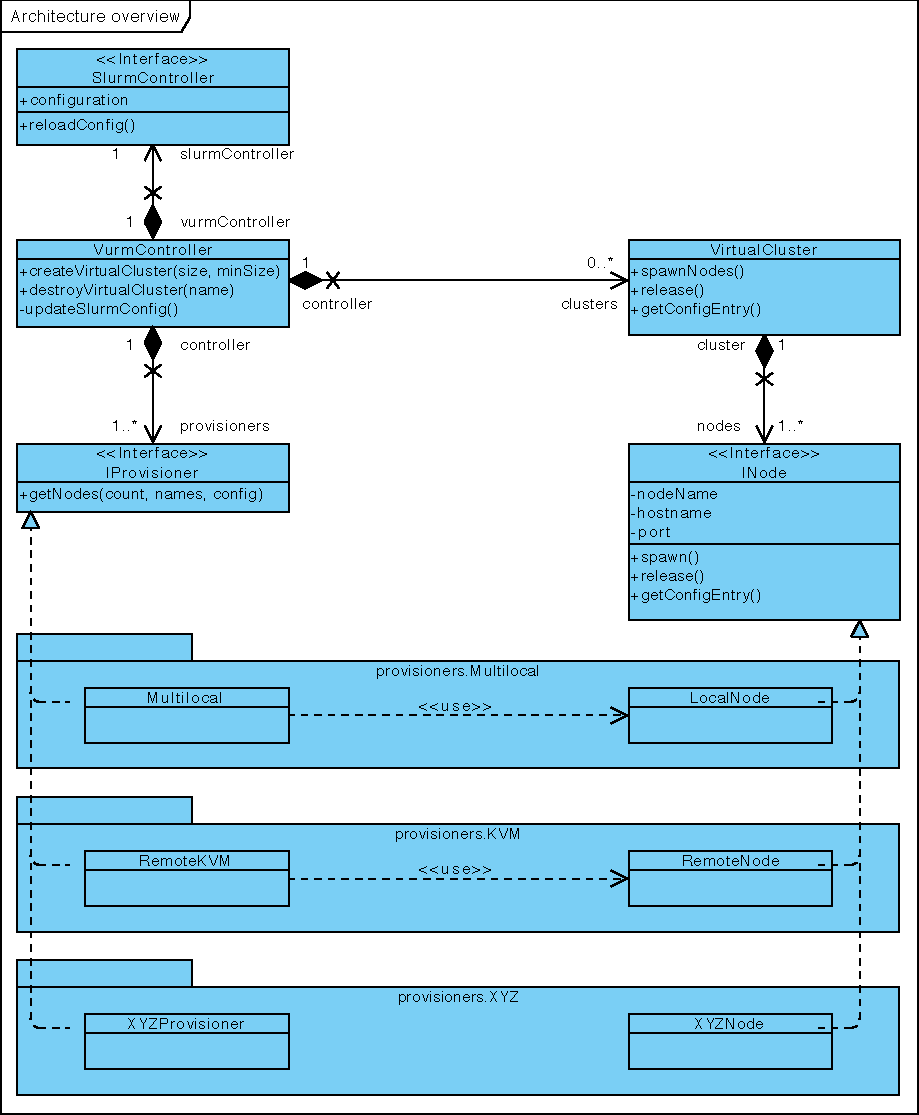
\includegraphics[width=.7\textwidth]{figures/arch-class}
	\caption{VURM architecture class diagram}
	\label{fig:arch-class}
\end{figure}

Each \texttt{IProvisioner} realization is a factory for objects providing the \texttt{INode} interface. The \texttt{VurmController} instance queries each registered \texttt{IProvisioner} realization instance for a given number of nodes, assembles them together and creates a new \texttt{VirtualCluster} instance.

Thanks to the complete abstraction of the \texttt{IProvisioner} and \texttt{INode} implementations, it is possible to use heterogeneous resource origins together as long as they implement the required interface. This makes easy to add new provisioner types (illustrated in the diagram by the \texttt{provisioners.XYZ} placeholder package) to an already existing architecture.

More details on the exact provisioning and virtual cluster creation process are given in the next section.

\section{Provisioning workflow}
\label{sec:vc-creation}

This section aims to introduce the concept of \emph{virtual cluster} and explain the provisioning workflow anticipated in the previous sections in deeper detail. Most of the explications provided in this section refer to the sequence diagram illustrated in \autoref{fig:provisioning} on page \pageref{fig:provisioning}.

\subsection{\emph{Virtual cluster} definition}

A \emph{virtual cluster} is a logical grouping of virtual machines spawned in response to a user request. \glspl{vm} in a virtual cluster belong to the user which initially requested them and can be exploited to run batch jobs through \gls{slurm}. These nodes can originate from different providers, depending on the particular resource availability when the creation request occurs.

Virtual clusters are exposed to \gls{slurm} as normal partitions containing all virtual nodes assigned to the virtual cluster. The \gls{vurm} controller modifies the \gls{slurm} configuration by placing the nodes and partition definition between comments clearly identifying each virtual cluster and allowing an automated process to retrieve the defined virtual clusters by simply parsing the configuration. An example of such a configuration for a virtual cluster consisting of two nodes is illustrated in \autoref{lst:vc-config}.

\lstset{language=bash,caption=SLURM configuration for a virtual cluster,label=lst:vc-config}
\begin{lstlisting}
# [vc-6ad4185]
NodeName=nd-6ad4185-0 NodeHostname=10.0.0.101
NodeName=nd-6ad4185-1 NodeHostname=10.0.0.100
PartitionName=vc-6ad4185 Nodes=nd-6ad4185-[0-1] Default=NO MaxTime=INFINITE State=UP
# [/vc-6ad4185]
\end{lstlisting}

Once a virtual cluster is created, the user can run jobs on it by using the \texttt{-{}-partition} argument to the \texttt{srun} command, as illustrated in the \autoref{lst:run-partition}.

\lstset{language=bash,caption=Batch job execution on a virtual cluster,label=lst:run-partition}
\begin{lstlisting}
# The -N2 argument forces SLURM to execute the job on 2 nodes
srun --partition=vc-6ad4185 -N2 hostname
\end{lstlisting}

The introduction of the concept of \emph{virtual cluster} allows thus to manage a logical group of nodes belonging to the same allocation unit, conveniently mapped to a \gls{slurm} partition, and enables the user to access and exploit the resources assigned to him in the best possible way.

\subsection{Virtual cluster creation}

A new virtual cluster creation process is started as soon as the user executes the newly provided \texttt{valloc} command. The only required parameter is the desired size of the virtual cluster to be created. Optionally, a minimal size and the priority can also be specified. The minimum size will be used as the failing threshold if the controller can't find enough resources to satisfy the requested size. If not specified, the minimum size defaults to the canonical size (message 1 in the sequence diagram in the \autoref{fig:provisioning}). The priority (defaulting to 1) is used to allocate resources to the virtual cluster and is further described in \autoref{sec:migration}, starting at page \pageref{sec:migration}.

When a request for a new virtual cluster is received, the controller asks the first defined provisioner for the requested amount of nodes. The provisioner can decide, based on the current system load, to allocate and return all nodes, only a part of them or none at all (messages 1.1, 1.2 and 1.2.1).

Until the total number of allocated nodes does not reach the requested size, the controller goes on by asking the next provisioner to allocate the remaining number of nodes. If the provisioners list is exhausted without reaching the user-requested number of nodes, the minimum size is checked. In the case that the number of allocated nodes equals or exceeds the minimum cluster size, the processing goes on; otherwise all nodes are released and the error propagated back to the user.

\needspace{5\baselineskip}
\noindent\rule[.15em]{10pt}{.3pt} \textbf{\tiny NOTE }{\leaders\hbox{\rule[.15em]{1pt}{.3pt}}\hfill}
\\[1mm]
The \texttt{loop} block with the alternate \texttt{opt} illustrated in the sequence diagram (first block) equals to the Python-specific \texttt{for-else} construct. In this construct, the \texttt{else} clause is executed only if the \texttt{for}-loop completes all the iterations without executing a \texttt{break} statement.

The Python documentation explaining the exact syntax and semantics of the \texttt{for-else} construct can be found at the following url: \url{http://docs.python.org/reference/compound_stmts.html#for}

In this specific case, the \texttt{else} clause is executed when the controller – after having iterated over all provisioners – has not collected the requested number of nodes.\\
\vspace{-4mm}\rule{\textwidth}{.3pt}
\vspace*{1mm}

Once the resource allocation process successfully completes, a new virtual cluster instance is created with the collected nodes (message 1.5) and the currently running \gls{slurm} controller is reconfigured and restarted (messages 1.6 and 1.7).

At this point, if the reconfiguration operation successfully completes, a \gls{slurm} daemon instance is spawned on each node of the virtual cluster (messages 2 and 2.1). If the reconfiguration fails, instead, the virtual cluster is destroyed by releasing all its nodes (messages 3 and 3.1) and the error is propagated back to the user.

If all the operations complete successfully, the random generated name of the virtual cluster is returned to the user to be used in future \texttt{srun} or \texttt{vrelease} invocations.

\begin{figure}[p]
	\centering
	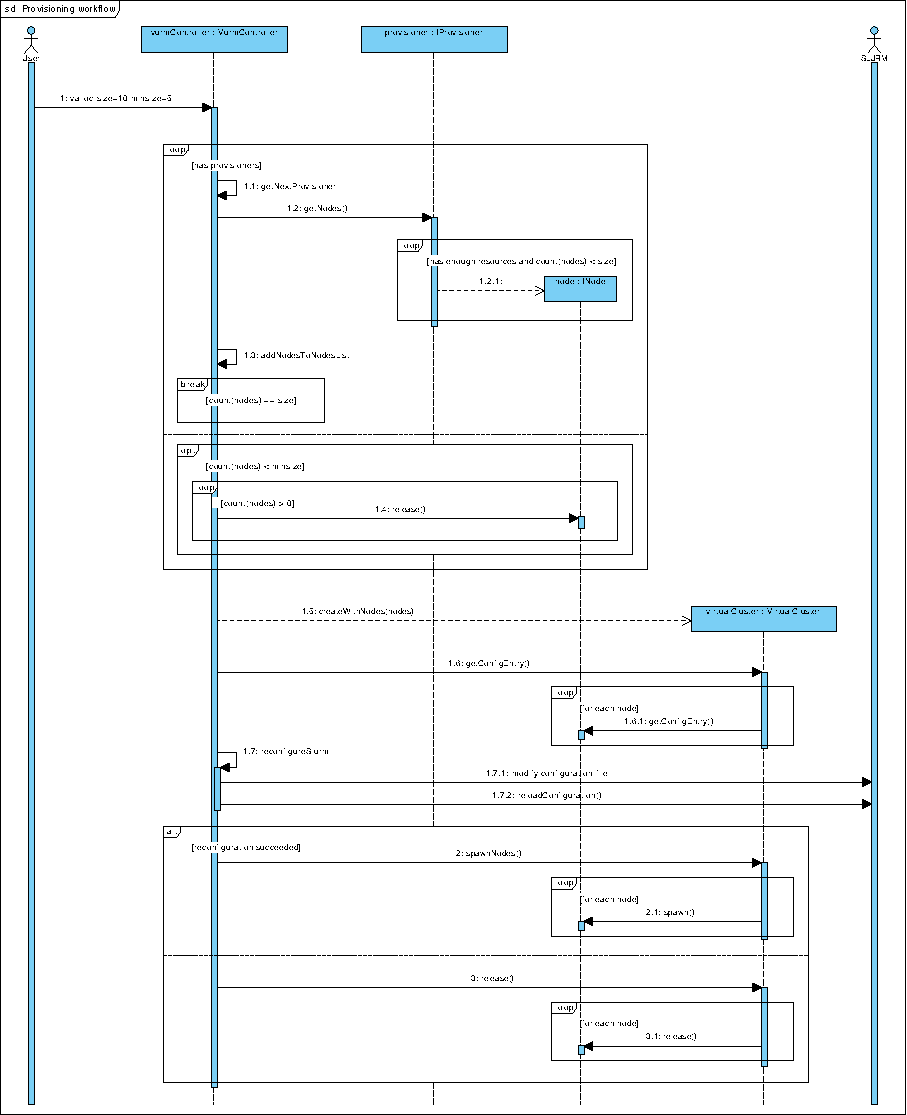
\includegraphics[width=1\textwidth]{figures/provisioning-workflow}
	\caption{Resource provisioning workflow}
	\label{fig:provisioning}
\end{figure}


\section{Implementing new provisioners}
\label{sec:new-provisioners}

The default implementation ships with two different provisioner implementations: the \texttt{multilocal} implementation is intended for testing purposes and spawns multiple \gls{slurm} daemons with different names on the local node while the \texttt{remotevirt} implementation runs \gls{slurm} daemons on virtual machines spawned on remote nodes (the \texttt{remotevirt} implementation is explained in further detail in \autoref{sec:remotevirt}: \emph{\nameref{sec:remotevirt}}, starting at page \pageref{sec:remotevirt}).

It is possible to easily add new custom provisioners to the \gls{vurm} controller by implementing the \texttt{IProvisioner} interface and registering an instance of such class to the \texttt{VurmController} instance. The \autoref{lst:custom-provisioner} describes how a custom provisioner instance providing the correct interface can be registered to the \gls{vurm} controller instance.

\lstset{language=python,caption=\texttt{vurm/bin/vurmctld.py},label=lst:custom-provisioner,firstnumber=40}
\begin{lstlisting}
# Build controller
ctld = controller.VurmController(config, [
    # Custom defined provisioner
    #  Instantiate and configure the custom provisioner directly here or
    #  outside the VurmController constructor invocation.
    #  If the custom provisioner is intended as a fallback provisioner,
    #  put it after the main one in this list.
    customprovisioner.Provisioner(customArgument, reactor, config),

    remotevirt.Provisioner(reactor, config),  # Default shipped provisioner
    multilocal.Provisioner(reactor, config),  # Testing provisioner
])
\end{lstlisting}
\lstset{firstnumber=1}

One of the future improvements foresees to adopt a plugin architecture to implement, publish and configure the provisioners; refer to the conclusions chapter on page \pageref{sec:future} for more information about this topic.

